\documentclass[a4paper,10pt]{article}
\usepackage[utf8]{inputenc}
\usepackage{graphicx}

%opening

\title{Técnicas de Controle de Concorrência
}
\author{Augusto C. A. Ribas}

\begin{document}

\maketitle

\section{Considere as três transações T1, T2 e T3 e as schedules S1 e S2 dadas a seguir, aplique o algoritmo de ordenação por rótulos de tempo para as schedules acima e
determine se o algoritmo terminará a execução das mesmas.}

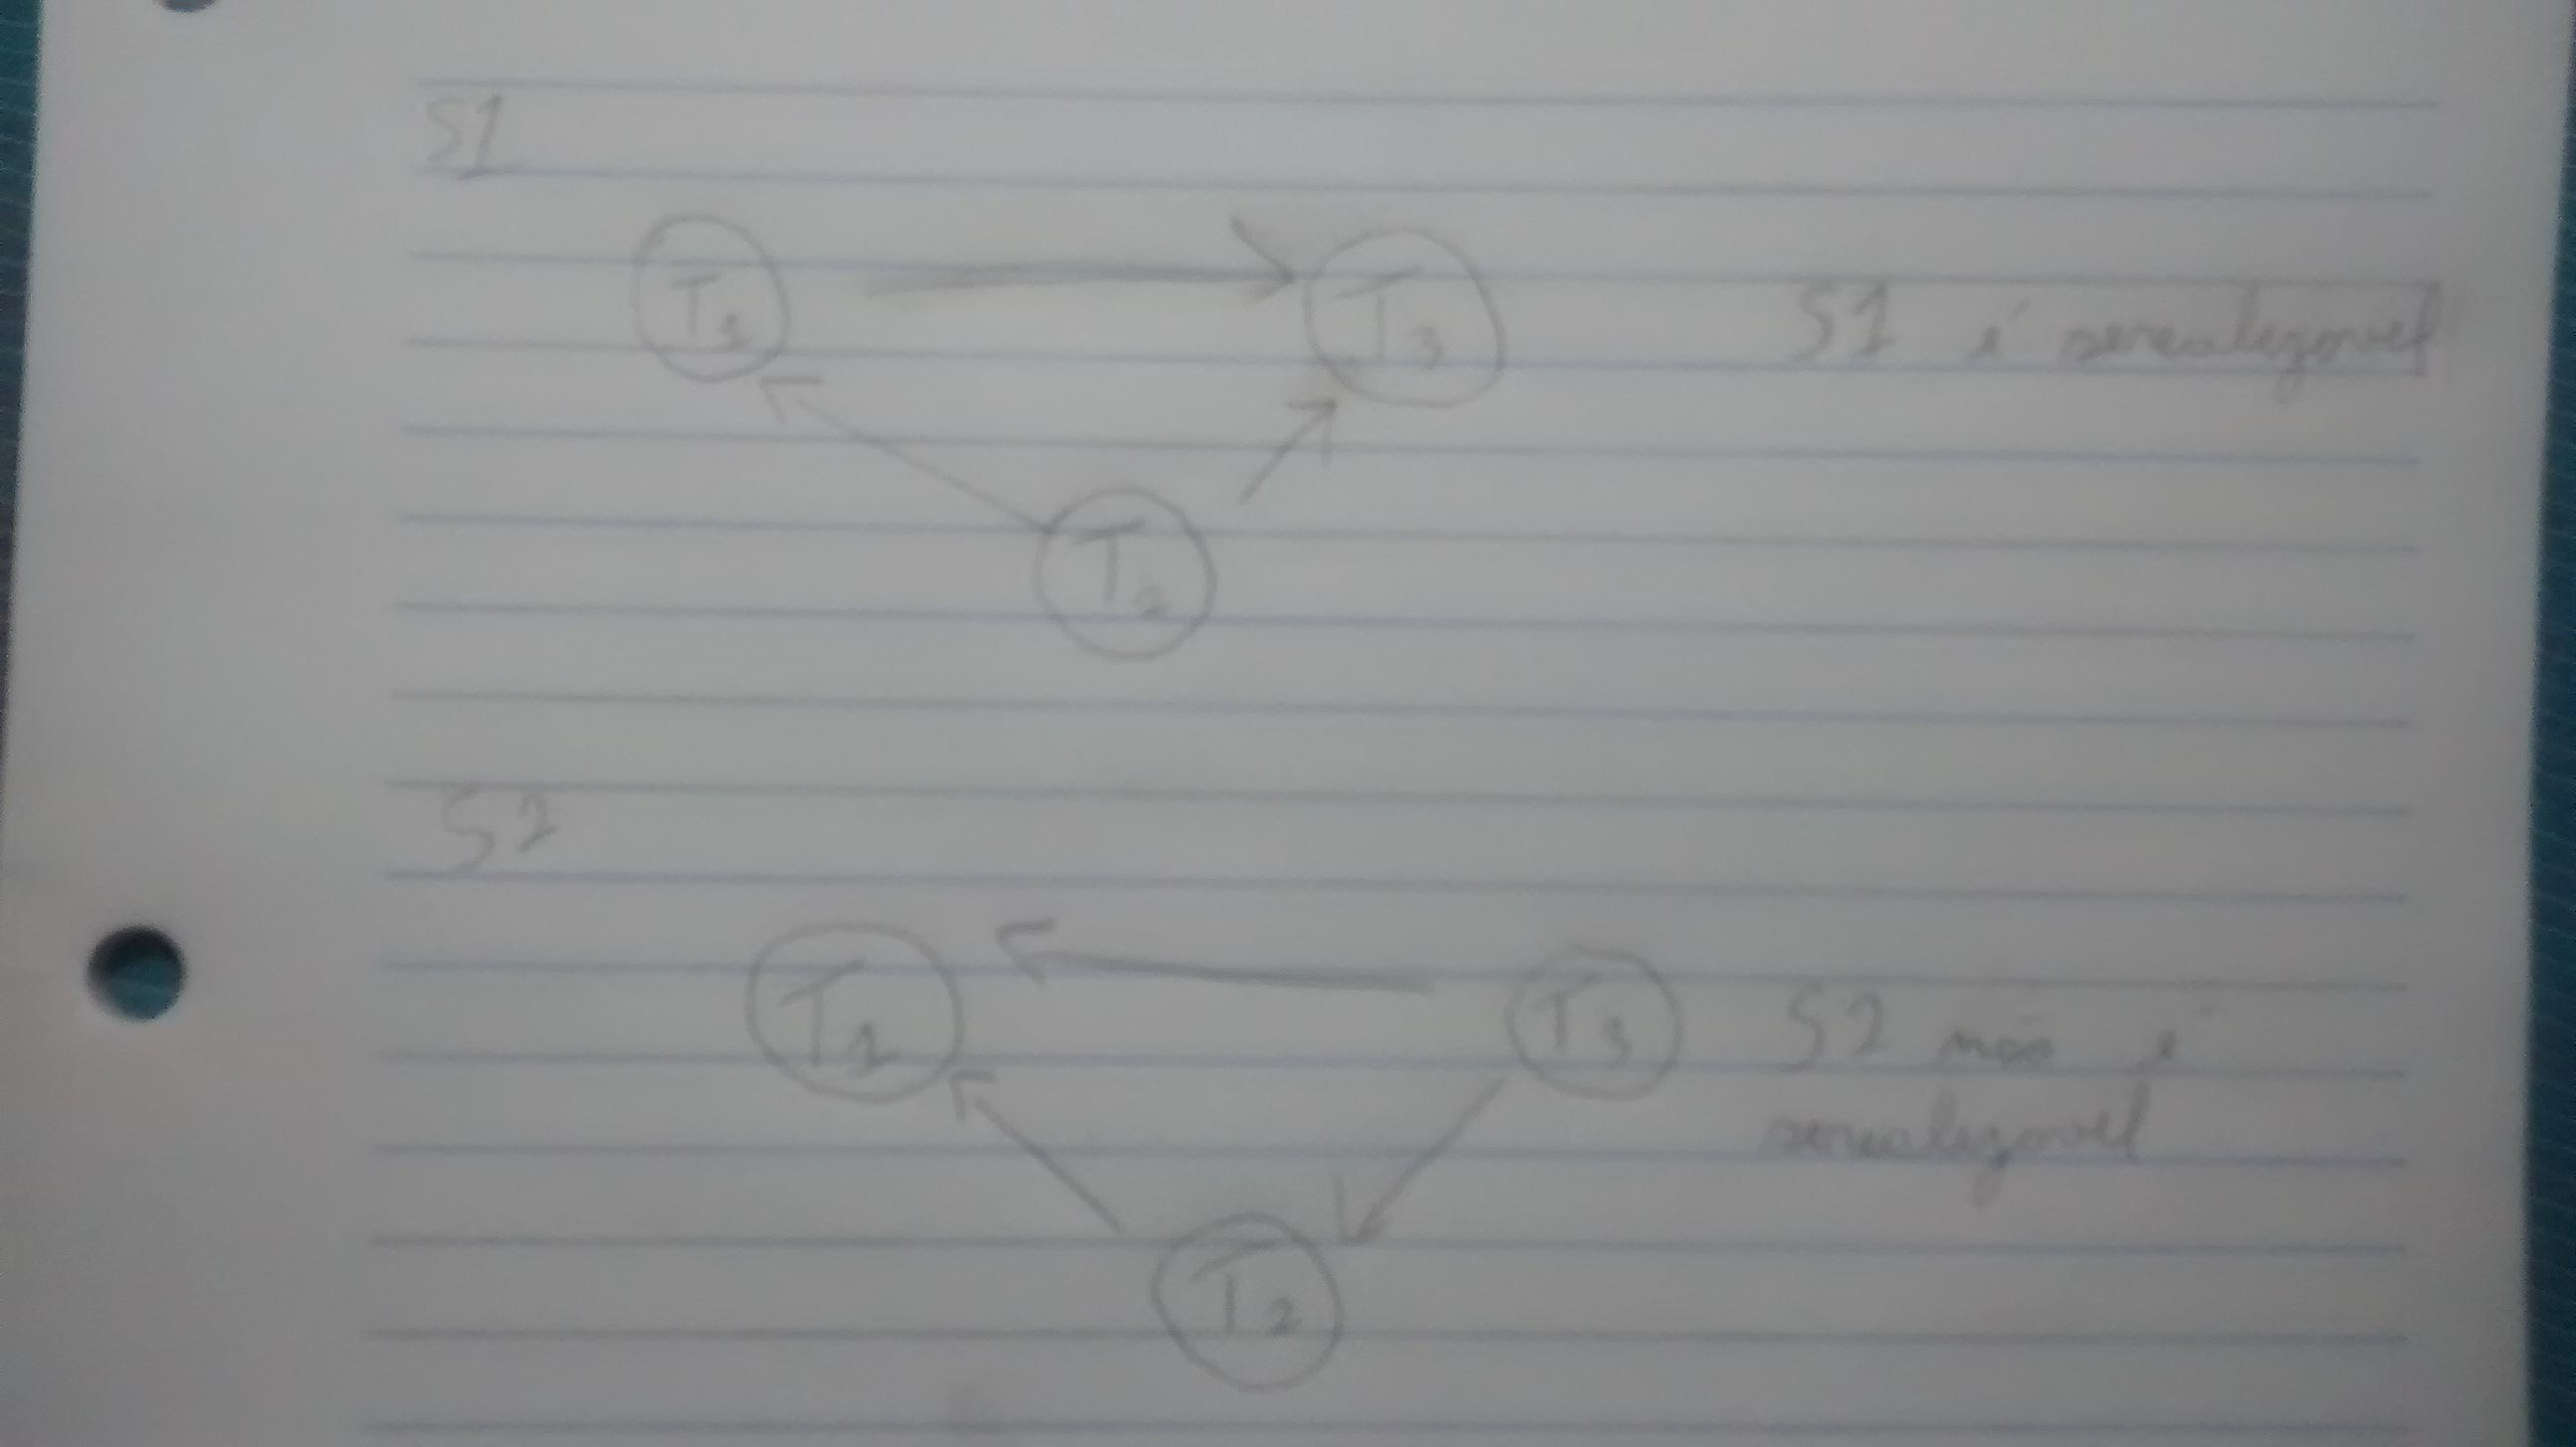
\includegraphics[width=1\textwidth]{IMG_20141105_214852194}

\section{O que é o protocolo de bloqueio em duas fases? Como ele garante a serialização?}
O protocolo de bloqueio em duas fases (2PL) é um método de controle de concorrência que garante a serialização. Ele utiliza bloqueios (locks) aplicados a transações, que podem bloquear outras transações de acessar partes de dados durante a vida de uma transação.
Basicamente o protocolo de bloqueio em duas fases é aplicado e removido em duas fases.

\begin{itemize}
\item Fase de expanção(Expanding phase): bloqueios (locks) são adquiridos e nenhum dado bloqueado é liberado.
\item Fase de encolhimento(Shrinking phase):bloqueios (locks) são liberados e nenhum novo bloqueio é feito.
\end{itemize}



\section{Discuta os problemas de deadlock e starvation (inanição) e as diferentes técnicas para lidar com esses problemas.}

Deadlocks ocorrem quando um transação $T_1$, em um grupo T de duas ou mais transações, esta esperando por outra transação, $T_2$ e esta por sua vez está esperando a transação $T_1$. Sendo que o deadlock pode ocorrer em qualquer número de transações, quando é gerado uma dependência circular entre estas.

Uma maneira de prevenir deadlock é usar algum protocolo de prevenção, como o bloqueio de duas fases conservador (conservative two-phase locking) que requer que todo bloqueio de  transação também bloquei todos os itens que vai precisar antes durante a aplicação do bloqueio, se algum dos itens não puder ser bloqueado, nenhum item é bloqueado, prevenindo deadlocks, mas fazendo com que a transação inteira espere por uma nova oportunidade de bloquear todos os itens, mas essa solução não é muito eficiente, ja que limita a concorrência de transações.
Outra possível solução envolve ordenar todos os itens do banco de dados garantindo que a transação que precisar de uma serie de itens vai bloquear todos eles de acordo com a ordem do banco de dados. Essa solução requer que a transação saiba a ordem dos itens que vai precisa, o que não é pratico no contexto de banco de dados. Na prática, o conceito de timestamp de tranção é usado.

Inanição (starvation) é outro problema comum com o uso de bloqueios (locks), e ocorrem quando uma transação não pode prosseguir por um período indefinido de tempo enquanto outras transações continuam normalmente no sistema. A inanição ocorre quando o esquema de bloqueios não é justo, isso é, dando prioridade para algum tipo de transação sobre outros.
Uma solução para a inanição é ter um sistema de espera justo, usando algum sistema como o fcfs (primeiro que chega é o primeiro a ser servido, first-come-first-served queue). Outro solução é usar um sistema que prioriza transações, mas aumenta a prioridade das transações de acordo com o tempo que elas esperam, garantindo que nenhuma transação vai esperar para sempre, não conseguindo terminar.

\section{Como a granularidade de itens de dados afeta o desempenho do controle de concorrência? Que fatores afetam a seleção do tamanho de granularidade para itens de dados?}

O tamanho dos itens de um banco de dados são chamados de granularidade de itens de dados e muitas relações de compromisso são estabelecidas para escolher esta granularidade.
Primeiro, quando maior a granularidade, menor a possibilidade de concorrência. Por exemplo, se o tamanho dos itens de dados são um bloco de disco, uma transação T que precisa bloquear um dado B precisa bloquear todo o bloco de disco onde esse dado está, bloqueando outros dados que também estão nesse bloco de disco e poderiam estar sendo usados sem problemas por outras transações. Se a granularidade fosse por dado, a transação T somente bloquearia o dado B que precisa, deixando outras informações daquele mesmo bloco de disco livre. Por outro lado, quanto menor o tamanho do item, maior o número de itens no banco de dados. Como todo item é associado a uma chave(para o bloqueio), o sistema vai precisar de um grande numero de chaves para administrar os bloqueis. Mais operações de bloqueio deveram ser realizadas e o sistema tera que administrar está operações, pode levar a uma sobrecarga do sistema dependendo da granularidade dos itens, além de gastar mais espaço com a tabela de bloqueios.

Assim, a resposta para qual tamanho ótimo de granularidade depende do tipo de transação envolvida. Se uma transação comum acessa um pequeno numero de registros, compensa ter uma granularidade de um registro de dados, mas se uma transação tipicamente acessa muitos registros de um mesmo arquivo, pode ser mais vantajoso acessar ter uma granularidade de bloco ou arquivo, já que a transação vai considerar todos os registros que quer acessar como um item de dados.

\end{document}
